%!TEX root = /lecture/Discrete_Optimistic.tex

\begin{theorem}\label{thm:gap3sat}
    $ \forall \epsilon>0 $,  $ \mathrm{GAP-3SAT}_{1,\frac{7}{8}+\epsilon} $ is NP-Hard.  
\end{theorem}
\begin{corollary}
    $ \forall \epsilon>0 $,  $ (\frac{7}{8}+\epsilon) $-approximation Max3SAT is NP-Hard. 
\end{corollary}

The corollary is equivalent to  $ \forall \epsilon>0,\mathrm{Gap3SAT}_{1-\epsilon,\frac{7}{8}+\epsilon} $ is NP-Hard.

\begin{remark}
    It implies that  it is hard to find an algorithm better than random algorithm. It also shows that perfect completeness is sometimes very hard.
\end{remark}

\subsection{Label-Cover Games}

To prove the theorem, we need to consider a constraint Graph  $ G=(U,V,E) $, which is a bipartite graph. 

\underline{Prover} is a function  $ \sigma:U\rightarrow [K],V\rightarrow [L] $. 

\underline{Constraints}: For each  $ e=(u,v)\in E $,  $ \pi_e:[L]\rightarrow [K] $.

\underline{Verifier}: Uniformaly sample  $ e=(u,v)\in  E $, accepts only if  $ \pi_e(\sigma(v))=\sigma(u) $.

The system is also called  "2-Prover-1Verifier  Game" or "Projection Game".

More generally,  $ \pi_e\subset [K]\times [L] $.

\begin{claim}
    PCP Theorem implies that  $ \exists \delta>0 $,  $ \mathrm{Gap-LC}_{1,1-\delta}^{(K,L)=(2,7)} $ is NP-Hard.  
\end{claim}
\begin{proof}
    Reduce from  $ \mathrm{Gap-3SAT}_{1,1-\epsilon} $. 

        \begin{center}
        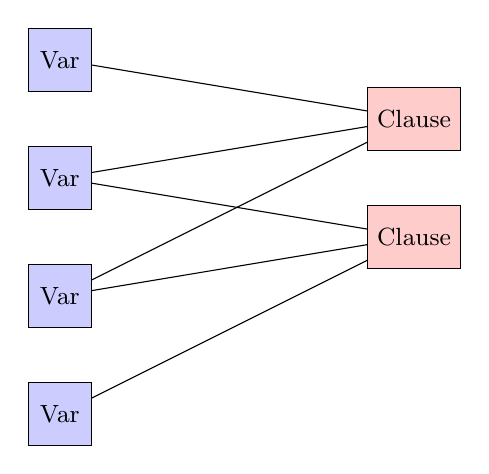
\begin{tikzpicture}[scale=1.5, every node/.style={draw, minimum size=0.8cm, font=\small}]
            % Variables (U)
            \node[fill=blue!20] (x1) at (0, 2) {Var};
            \node[fill=blue!20] (x2) at (0, 1) {Var};
            \node[fill=blue!20] (x3) at (0, 0) {Var};
            \node[fill=blue!20] (x4) at (0, -1) {Var};

            % Clauses (V)
            \node[fill=red!20] (c1) at (3, 1.5) {Clause};
            \node[fill=red!20] (c2) at (3, 0.5) {Clause};

            % Edges
            \draw[-] (x1) -- (c1);
            \draw[-] (x2) -- (c1);
            \draw[-] (x3) -- (c1);
            \draw[-] (x2) -- (c2);
            \draw[-] (x3) -- (c2);
            \draw[-] (x4) -- (c2);
        \end{tikzpicture}
        \end{center}

        Variables  $ x_i $ have  $ \sigma(x_i)\in \{0,1\} $ and Clauses  $ c_i=x_{j_i}^1\wedge x_{j_i}^2\wedge x_{j_i}^3 $ have  $ \sigma(c_i)\in [7] $ to represent the state of  $ c_i $.
    \end{proof}

\subsubsection{Paralled Repetition}
Given  $ H=\left(G(U,V,E),K,L,\{\pi_e\}\right) $.
\[H^{\otimes t}=\left(G^{\otimes t},K^t,L^t,\{\pi_{e_1,e_2,\cdots,e_t}\}\right)\]
where 
\[G^{\otimes t}=\{(u_1,u_2,\cdots,u_t),(v_1,v_2,\cdots,v_T)\}\] 

\[\pi_{(u_1,v_1),\cdots,(u_t,v_t)}=\left\{\left((\alpha_1,\cdots,\alpha_t),(\beta_1,\cdots,\beta_t)\right):(\alpha_i,\beta_i)\in \pi_{(u_i,v_i)}\right\}\]

It is easy to check that if  $ H  $ is a projection game,  $ H^{\otimes t} $ is also a projection game.

We wonder whether the following theorem holds
\begin{theorem}[not quite true]
    \[\OPT(H^{\otimes t}) \leq \OPT(H)^t\]
\end{theorem}
There is a counter-example for  $ U=\{u_1,u_2\},V=\{v_1,v_2\},K=L=4 $ and  $ G $ is fully connected. 
$ [K],[L]\leftrightarrow \{u,v\}\times\{1,2\} $ 

$ \pi_{(u_i,v_j)}=\{((u,i),(u,i)),((v,j),(v,j))\} $ 

Clearly,  $ \OPT(H)=\frac{1}{2} $.

However,  $ \OPT(H^{\otimes 2})=\frac{1}{2} $.

Let  $ \sigma((u_{i_1},u_{i_2}))=(((u,i_1),(v,i_1))) $,  $ \sigma((v_{j_2},v_{j_2}))=((u,j_1),(v,j_2)) $.  

So verifier accepts if  $ i_1=j_2 $.

However, the following theorem holds:
\begin{theorem}
    Suppose  $ H  $ has alphabet size less than  $ k $ and  $ \OPT(H) \leq 1-\delta $.  Then 
    \[\OPT(H^{\otimes t}) \leq \exp(-\Omega(\frac{\delta^3t}{\log K}))\]  
\end{theorem}
\begin{corollary}\label{LC large theorem}
    $ \forall \delta>0 $,  $ \exists  $   $ K,L $ such that  $ \mathrm{GAP-LC}(K,L)_{1,\delta} $ is NP-Hard.  
\end{corollary}
In fact, the above hardness still holds even when the constraints graph is regular and (and  $ |U|=|V| $) 